\documentclass[All.tex]{subfiles}
%%---------------------------%
%%---- Обычный файл      ----%
%%---------------------------%
%\sloppy
%\documentclass[14pt,a4paper,oneside]{extarticle}	% Размер основного шрифта и формата листа
%\usepackage{xltxtra}						% Используется для вывода логотипа XeLaTeX
%\usepackage{xunicode}						% Кодировка документа
%\usepackage{polyglossia}					% Загружает пакет многоязыковой верстки
%\newfontfamily\russianfont{Book Antiqua}
%%\setmainfont{Liberation Serif}						% Основной шрифт текста
%\setmainfont{Book Antiqua}
%\setdefaultlanguage{russian}				% Основной язык текста
%\setotherlanguage{english}					% Дополнительный язык текста
%\linespread{1}							% Межстрочный интервал выбран полуторным
%\usepackage[left=2.5cm,
%right=1.5cm,vmargin=2.5cm]{geometry} % Отступы по краям листа
%\bibliographystyle{ugost2008}
%
%\usepackage{xcolor}
%\usepackage{hyperref}
%% Цвета для гиперссылок
%\definecolor{linkcolor}{HTML}{359B08} % цвет ссылок
%\definecolor{urlcolor}{HTML}{799B03} % цвет гиперссылок
%\hypersetup{pdfstartview=FitH,  linkcolor=linkcolor,urlcolor=urlcolor, colorlinks=true}
%
%%---------------------------%
%%---- Пакеты расширений ----%
%%---------------------------%
%\usepackage{xcolor}
%\usepackage{hyperref}
%% Цвета для гиперссылок
%\definecolor{linkcolor}{HTML}{359B08} % цвет ссылок
%\definecolor{urlcolor}{HTML}{799B03} % цвет гиперссылок
%\hypersetup{pdfstartview=FitH,  linkcolor=linkcolor,urlcolor=urlcolor, colorlinks=true}
%
%
%\usepackage{verbatim,indentfirst}
%\usepackage{cite,enumerate,float}
%\usepackage{amsmath,amssymb,amsthm,amsfonts}
%
%%---------------------------%
%%--- Вставка иллюстраций ---%
%%---------------------------%
%\usepackage{graphicx}
%\usepackage{subfigure}
%%\graphicspath{{Images/}}
%\usepackage{fontspec}

\begin{document}
%	\pagestyle{empty} %  выключаенм нумерацию
	%\setcounter{page}{3}% Нумерация начинается с третьей страницы
	%\renewcommand{\contentsname}{\center{Содержание}}
	%\tableofcontents

\chapter{\textcolor{PineGreen}{Динамика твердого тела}}
		%\addcontentsline{toc}{section}{Опыт 16. Нахождение центра масс}
		\section{Отыскание центра масс}

	
	\begin{figure}[H] 	
		\centering 	
		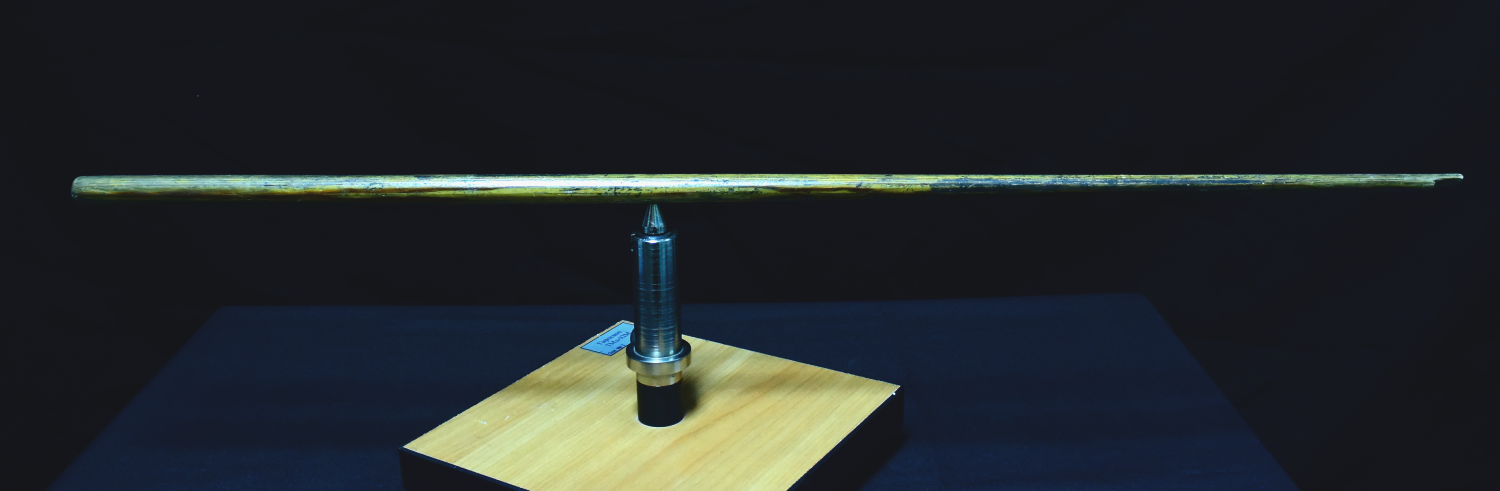
\includegraphics[width=0.9\linewidth]{center-1.png}
		\caption{Демонстрация одного из способов нахождения центра масс, основанного на свойствах сухого трения}
		\label{center-1}
	\end{figure}
	
	\subsection*{\textcolor{PineGreen}{Оборудование}}
	
	\begin{enumerate} 
		\item Протяженный предмет переменной толщины — указка с дециметровыми делениями или линейка.
	\end{enumerate}

\subsection*{\textcolor{PineGreen}{Основные определения}}
	
Центр масс — центр инерции, геометрическая точка, положение которой характеризует распределение масс в теле или механической системе. 
Координаты центра масс определяются формулами
$$
	x_c =\sum \dfrac{m_i x_i}{M}, y_c =\sum \dfrac{m_i y_i}{M}, z_c =\sum \dfrac{m_i z_i}{M},
$$
	или для тела при непрерывном распределении масс
$$
	x_c = \dfrac1M \int \rho x dV, y_c =\dfrac1M \int \rho y dV, z_c =\dfrac1M \int \rho z dV,
$$
	где $ m_i $ — массы материальных точек, образующих систему, $ x_i $, $ y_i $, $ z_i $ — координаты этих точек, $ M = \sum m_i $ — масса системы, $ \rho $ — плотность, \textit{V} — объем. 
	
	Понятие о центре масс отличается от понятия о центре тяжести тем, 
	что последнее имеет смысл только для твердого тела, находящегося в поле тяжести;
	понятие же о центре масс не связано ни с каким силовым полем и имеет смысл для любой механической системы. 
	Для твердого тела в однородном поле тяжести положения центра масс и центра тяжести совпадают. 
	
\subsection*{\textcolor{PineGreen}{Краткое описание}}
	
В ходе демонстрации твердое тело (указка или линейка метровой длины) кладется на пальцы рук.
Затем пальцы начинают сдвигать к центру тела. Тело в процессе опыта остается неподвижным, перемещаются лишь руки экспериментатора.
В конечном счете место их соприкосновения произойдет в некоторой точке, которая и окажется центром масс тела.
Следует обратить внимание на то, что при плавном перемешении рук проскальзывание происходит только между одним пальцем и телом, в то время как тело движется вместе с другим пальцем, оставаясь неподвижным относительного него.

\subsection*{\textcolor{PineGreen}{Теория}}
		
		На тело, находящееся в гравитационном поле Земли, всегда действует сила тяжести \textit{M}\textbf{g}.
		Если рассмотреть протяженное тело, например, стержень, расположенный на двух опорах, то со стороны каждой опоры на тело будет действовать сила реакции $ \textbf{N}_1 $ и $ \textbf{N}_2 $ соответсвенно (рис.\ref{center-2},\textit{а}).
		В общем случае эти силы не равны между собой, например, если масса распределена в стержне неравномерно.
		
		\begin{figure}[H]
			\centering 	
			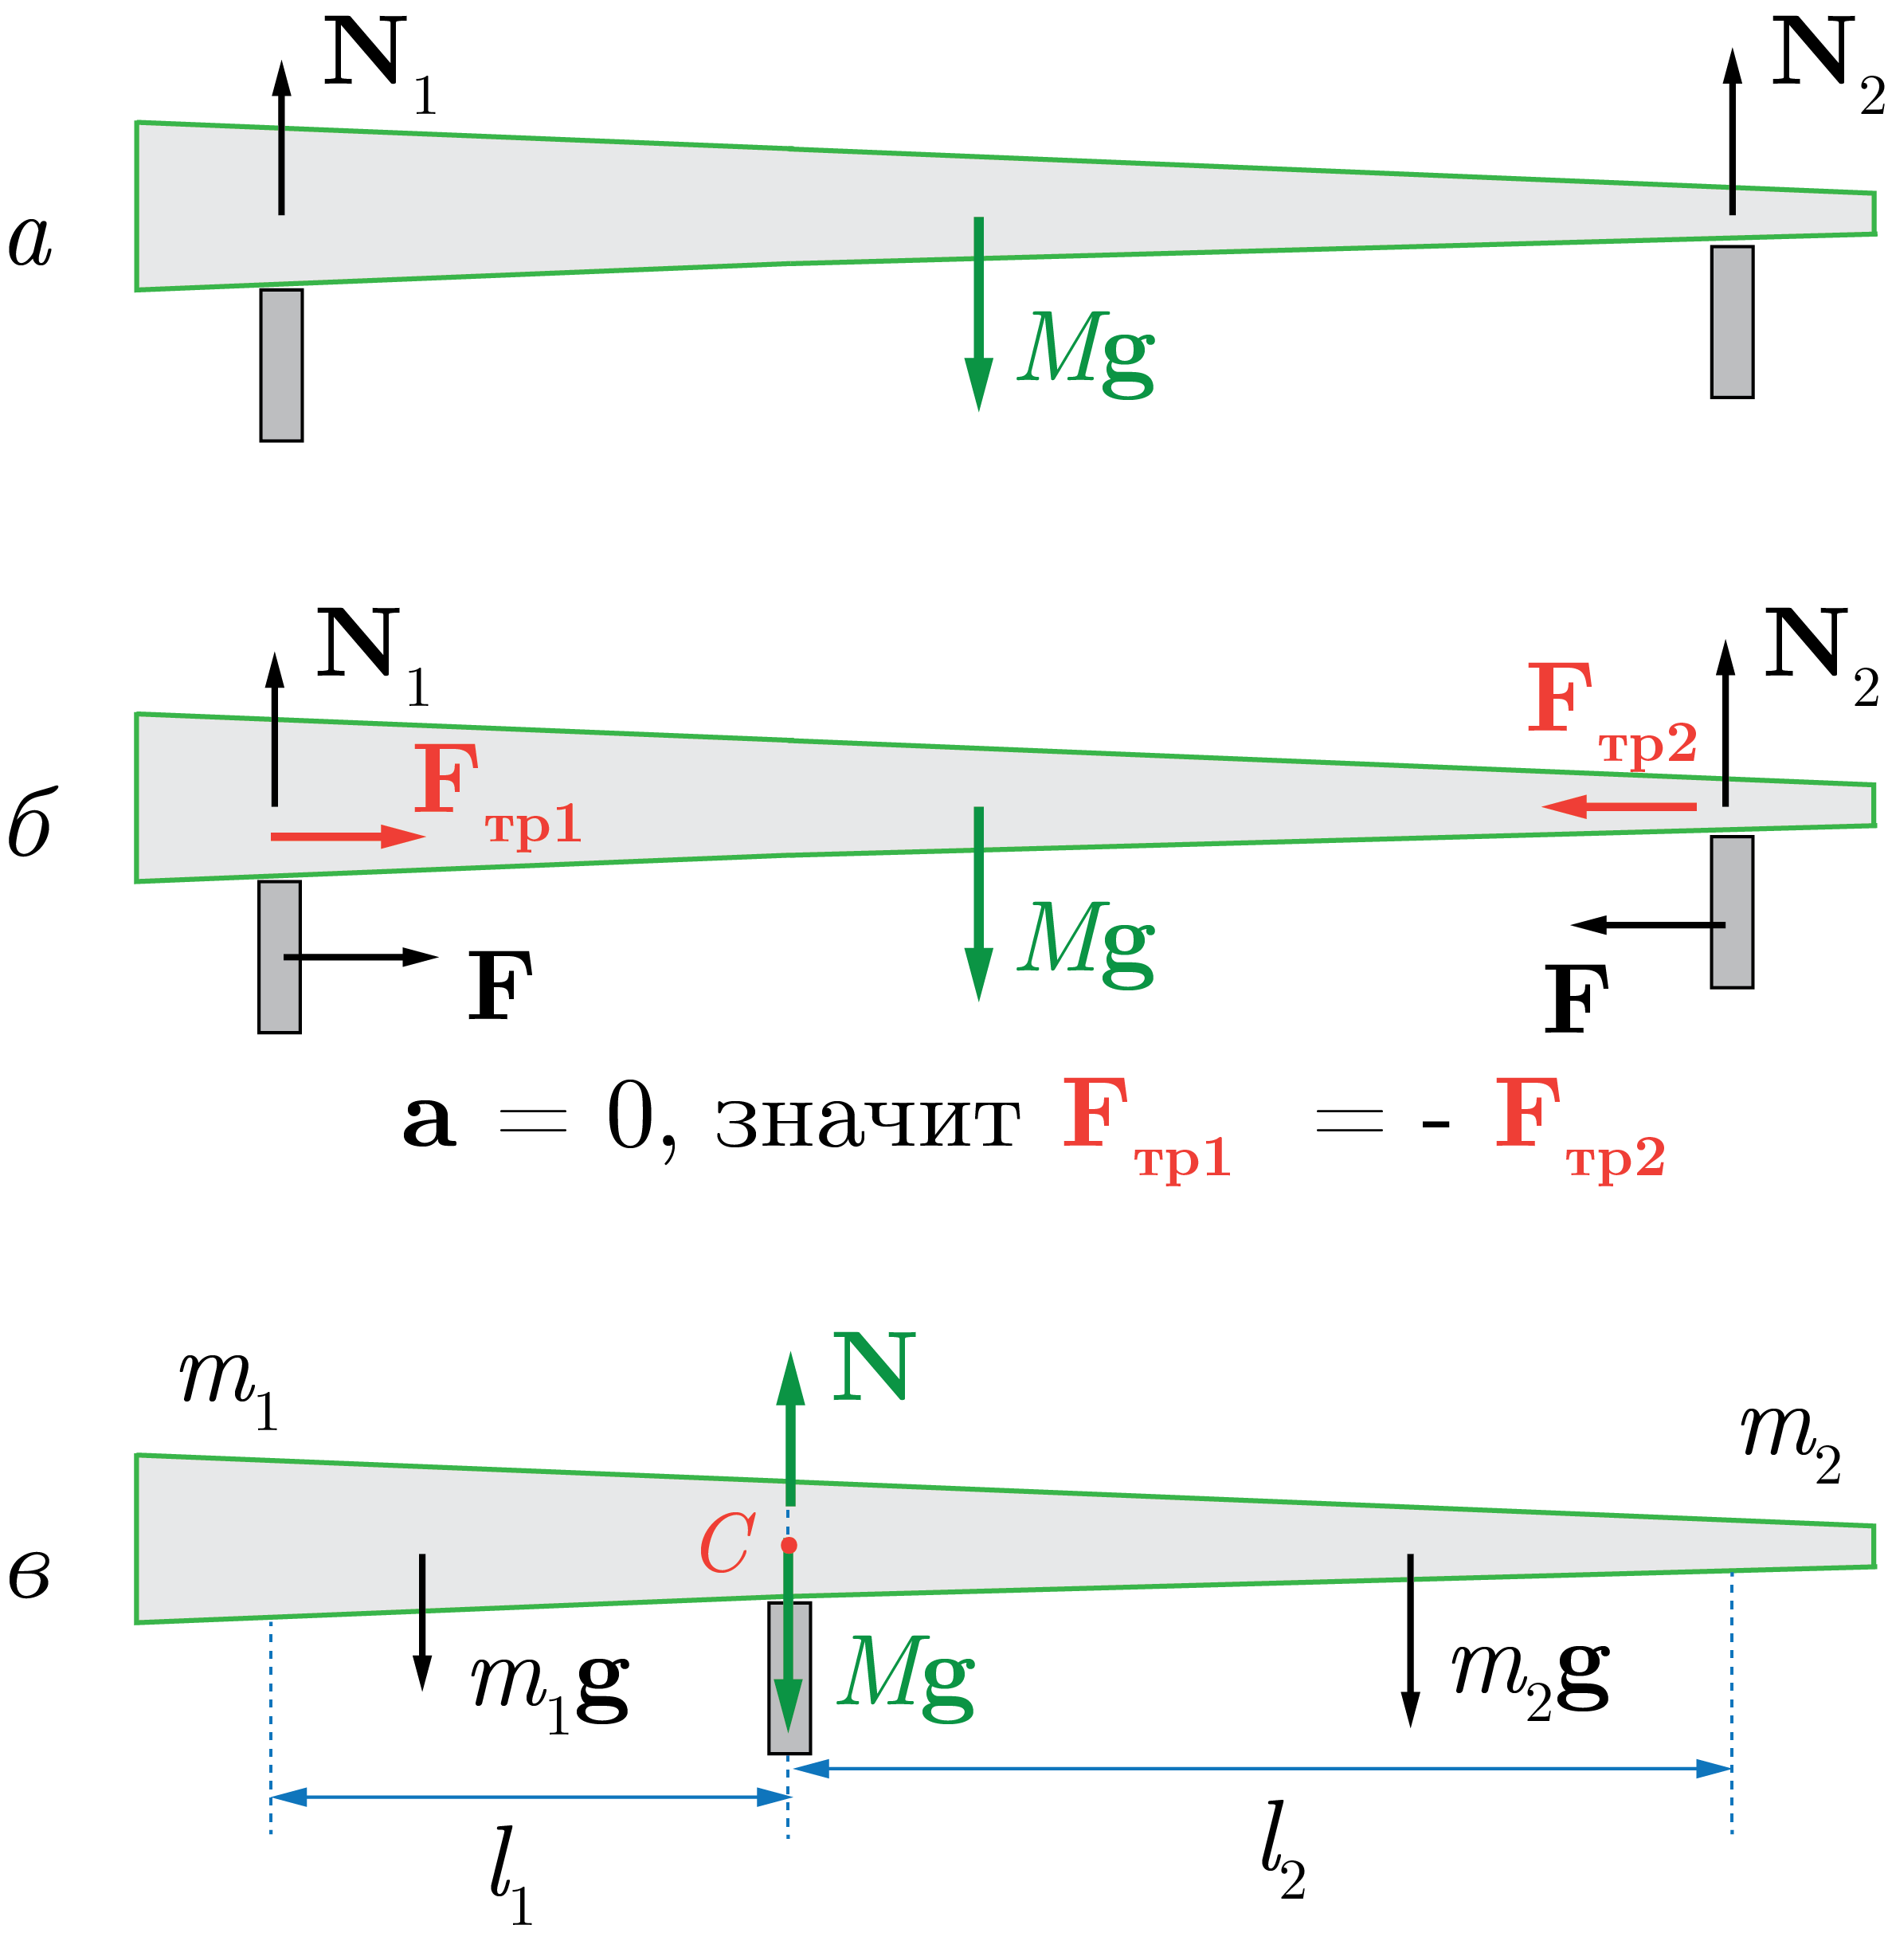
\includegraphics[width=0.55\linewidth]{center-2.png}
			\caption{Схематичное изображение твердого тела неправильной геометрической формы (\textit{а}). 
				положение центра масс такого тела определяется из условия его равновесия в однородном поле силы тяжести (\textit{б,в})}
			\label{center-2}
		\end{figure}
	
		Если опоры (пальцы рук) начнут сближаться, то между ними и телом возникнут силы трения $ \textbf{F}_{\text{тр}1} $ и $ \textbf{F}_{\text{тр}2} $ (рис.\ref{center-2},\textit{б}).
				
		Из условия, что стержень под действием сил трения и реакции опоры не изменяет своей скорости, следует:
		\begin{equation}
		a_c=0: \textbf{F}_{\text{тр}1} =\textbf{F}_{\text{тр}2}.
		\end{equation}	
		Сумма сил в вертикальном направлении обращается в нуль, а также сумма моментов сил относительно центра масс равна нулю:
		\begin{equation}
		\begin{cases}
		Mg = N_1 + N_2 \\
		N_1l_1 = N_2l_2.
		\end{cases}
		\end{equation}

Используя известную связь между силой трения и силой реакции опоры при скольжении тела, запишем равенство
\begin{equation}
\mu_1N_1 =\mu_2N_2,
\end{equation}
и соотношение
\begin{equation}
\dfrac{N_1}{N_2} =\dfrac{l_2}{l_1}.
\end{equation}
Таким образом, получим следующее выражение:
\begin{equation}
\dfrac{\mu_2}{\mu_1}=\dfrac{N_1}{N_2} =\dfrac{l_2}{l_1},
\end{equation}
откуда следует, что $ \mu_1 \neq \mu_2 $. В ходе эксперимента руки проскальзывают относительно тела попеременно, при этом в одной точке соприкосновения действует сила трения скольжения, в другой -- сила трения покоя. Полученное отношение коэффициентов трения $ \mu_1 $ и $ \mu_2 $ соответсвует соотношению коэффициентов трения скольжения и покоя, первый из которых, как правило, немного меньше второго.
\end{document}
